% Created by tikzDevice version 0.12 on 2019-02-14 20:19:28
% !TEX encoding = UTF-8 Unicode
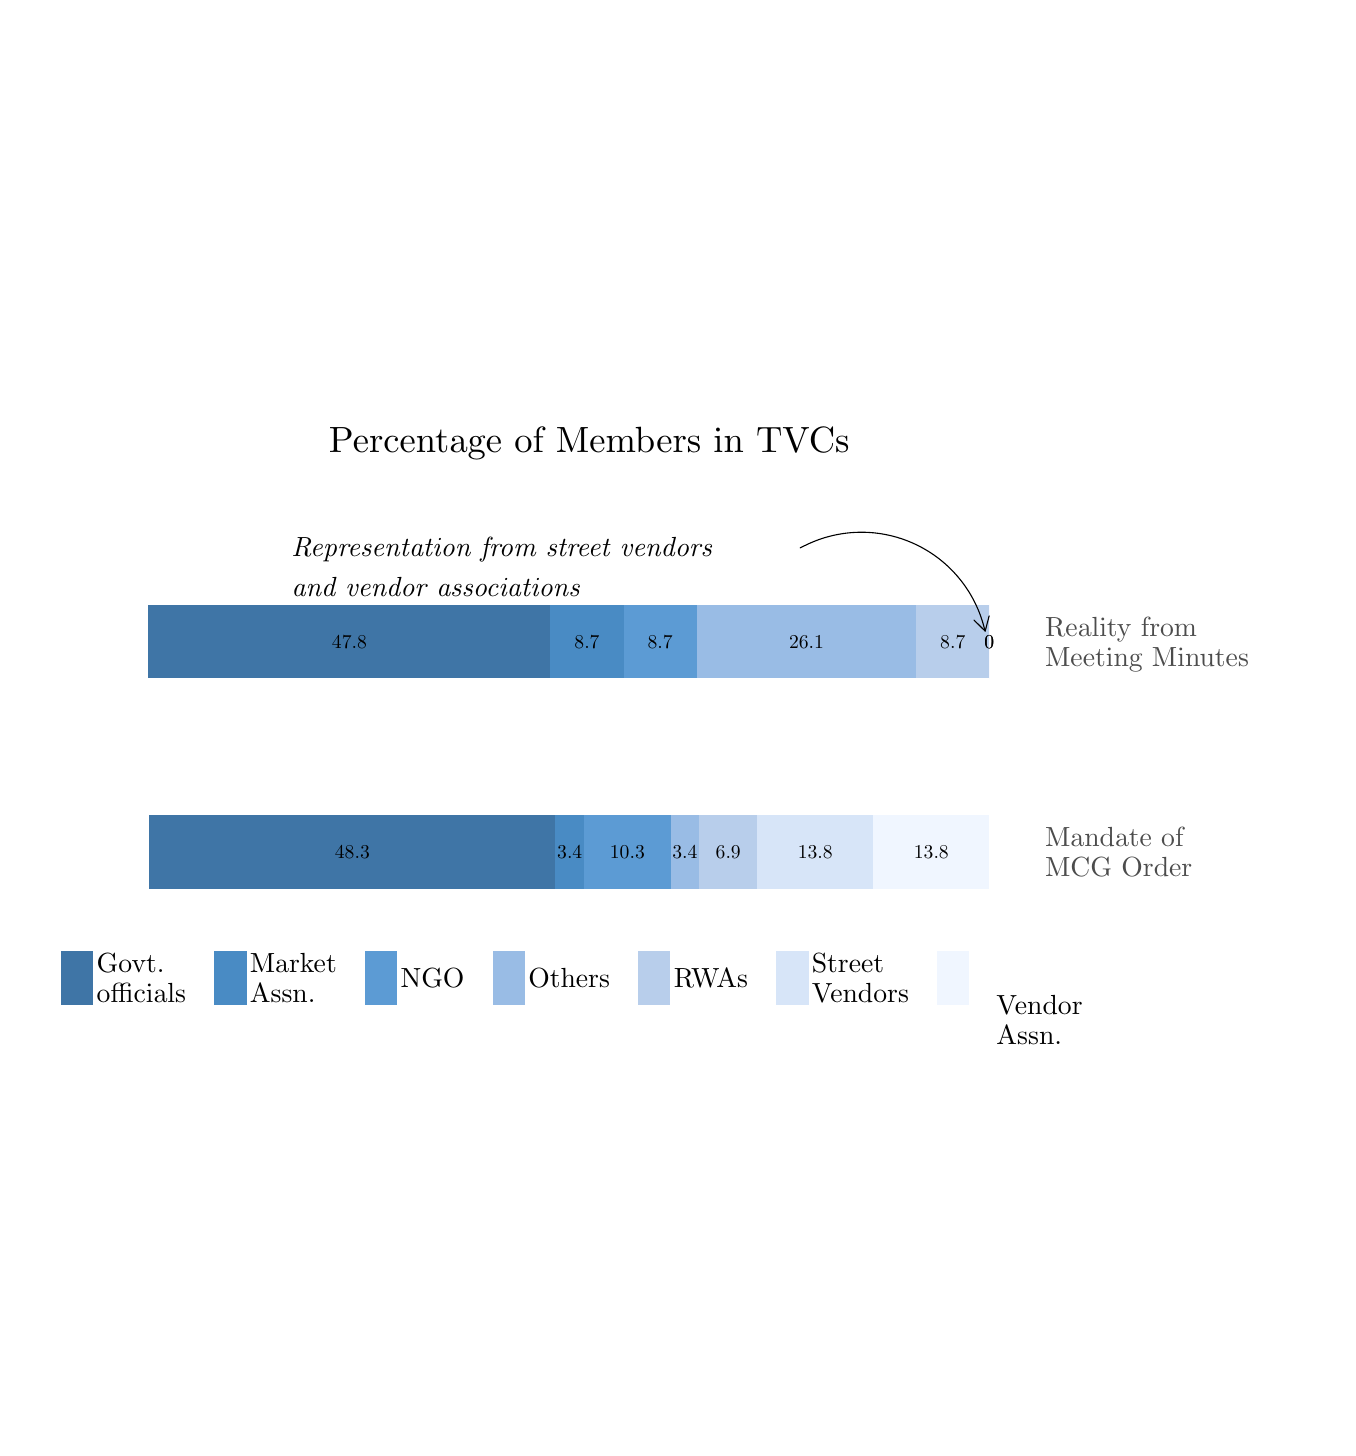
\begin{tikzpicture}[x=1pt,y=1pt]
\definecolor{fillColor}{RGB}{255,255,255}
\path[use as bounding box,fill=fillColor,fill opacity=0.00] (0,0) rectangle (469.75,505.89);
\begin{scope}
\path[clip] (  0.00,159.74) rectangle (469.75,346.15);
\definecolor{drawColor}{RGB}{255,255,255}
\definecolor{fillColor}{RGB}{255,255,255}

\path[draw=drawColor,line width= 0.6pt,line join=round,line cap=round,fill=fillColor] (  0.00,159.74) rectangle (469.76,346.15);
\end{scope}
\begin{scope}
\path[clip] ( 28.45,162.49) rectangle (362.70,329.62);
\definecolor{fillColor}{RGB}{240,246,255}

\path[fill=fillColor] (305.58,194.78) rectangle (347.51,221.36);
\definecolor{fillColor}{RGB}{215,229,248}

\path[fill=fillColor] (263.64,194.78) rectangle (305.58,221.36);
\definecolor{fillColor}{RGB}{184,206,235}

\path[fill=fillColor] (242.68,194.78) rectangle (263.64,221.36);
\definecolor{fillColor}{RGB}{153,188,229}

\path[fill=fillColor] (232.35,194.78) rectangle (242.68,221.36);
\definecolor{fillColor}{RGB}{92,155,212}

\path[fill=fillColor] (201.05,194.78) rectangle (232.35,221.36);
\definecolor{fillColor}{RGB}{73,139,196}

\path[fill=fillColor] (190.72,194.78) rectangle (201.05,221.36);
\definecolor{fillColor}{RGB}{63,117,166}

\path[fill=fillColor] ( 43.95,194.78) rectangle (190.72,221.36);
\definecolor{fillColor}{RGB}{184,206,235}

\path[fill=fillColor] (321.07,270.74) rectangle (347.51,297.33);
\definecolor{fillColor}{RGB}{153,188,229}

\path[fill=fillColor] (241.77,270.74) rectangle (321.07,297.33);
\definecolor{fillColor}{RGB}{92,155,212}

\path[fill=fillColor] (215.33,270.74) rectangle (241.77,297.33);
\definecolor{fillColor}{RGB}{73,139,196}

\path[fill=fillColor] (188.89,270.74) rectangle (215.33,297.33);
\definecolor{fillColor}{RGB}{63,117,166}

\path[fill=fillColor] ( 43.65,270.74) rectangle (188.89,297.33);
\definecolor{fillColor}{RGB}{240,246,255}

\path[fill=fillColor] (347.51,270.74) rectangle (347.51,297.33);
\definecolor{fillColor}{RGB}{215,229,248}

\path[fill=fillColor] (347.51,270.74) rectangle (347.51,297.33);
\definecolor{drawColor}{RGB}{0,0,0}

\node[text=drawColor,anchor=base,inner sep=0pt, outer sep=0pt, scale=  0.71] at (326.54,205.62) {13.8};

\node[text=drawColor,anchor=base,inner sep=0pt, outer sep=0pt, scale=  0.71] at (284.61,205.62) {13.8};

\node[text=drawColor,anchor=base,inner sep=0pt, outer sep=0pt, scale=  0.71] at (253.16,205.62) {6.9};

\node[text=drawColor,anchor=base,inner sep=0pt, outer sep=0pt, scale=  0.71] at (237.51,205.62) {3.4};

\node[text=drawColor,anchor=base,inner sep=0pt, outer sep=0pt, scale=  0.71] at (216.70,205.62) {10.3};

\node[text=drawColor,anchor=base,inner sep=0pt, outer sep=0pt, scale=  0.71] at (195.88,205.62) {3.4};

\node[text=drawColor,anchor=base,inner sep=0pt, outer sep=0pt, scale=  0.71] at (117.33,205.62) {48.3};

\node[text=drawColor,anchor=base,inner sep=0pt, outer sep=0pt, scale=  0.71] at (334.29,281.59) {8.7};

\node[text=drawColor,anchor=base,inner sep=0pt, outer sep=0pt, scale=  0.71] at (281.42,281.59) {26.1};

\node[text=drawColor,anchor=base,inner sep=0pt, outer sep=0pt, scale=  0.71] at (228.55,281.59) {8.7};

\node[text=drawColor,anchor=base,inner sep=0pt, outer sep=0pt, scale=  0.71] at (202.11,281.59) {8.7};

\node[text=drawColor,anchor=base,inner sep=0pt, outer sep=0pt, scale=  0.71] at (116.27,281.59) {47.8};

\node[text=drawColor,anchor=base,inner sep=0pt, outer sep=0pt, scale=  0.71] at (347.51,281.59) {0};

\node[text=drawColor,anchor=base,inner sep=0pt, outer sep=0pt, scale=  0.71] at (347.51,281.59) {0};

\path[draw=drawColor,line width= 0.4pt,line join=round,line cap=round] (279.14,317.92) --
	(279.33,318.01) --
	(280.18,318.43) --
	(281.24,318.94) --
	(282.09,319.34) --
	(282.79,319.66) --
	(283.49,319.96) --
	(284.25,320.27) --
	(285.06,320.59) --
	(285.84,320.88) --
	(286.55,321.13) --
	(287.27,321.37) --
	(288.06,321.61) --
	(288.90,321.85) --
	(289.69,322.07) --
	(290.43,322.26) --
	(291.17,322.43) --
	(291.98,322.61) --
	(292.83,322.77) --
	(293.64,322.92) --
	(294.39,323.04) --
	(295.15,323.15) --
	(295.97,323.25) --
	(296.83,323.34) --
	(297.65,323.42) --
	(298.41,323.47) --
	(299.17,323.51) --
	(300.00,323.54) --
	(300.86,323.56) --
	(301.69,323.56) --
	(302.45,323.55) --
	(303.21,323.52) --
	(304.03,323.48) --
	(304.90,323.42) --
	(305.72,323.35) --
	(306.48,323.27) --
	(307.23,323.17) --
	(308.05,323.06) --
	(308.91,322.92) --
	(309.72,322.78) --
	(310.47,322.63) --
	(311.21,322.47) --
	(312.02,322.29) --
	(312.86,322.07) --
	(313.66,321.86) --
	(314.39,321.65) --
	(315.11,321.42) --
	(315.90,321.17) --
	(316.72,320.88) --
	(317.49,320.60) --
	(318.20,320.32) --
	(318.91,320.03) --
	(319.67,319.71) --
	(320.46,319.35) --
	(321.20,319.00) --
	(321.89,318.66) --
	(322.56,318.32) --
	(323.29,317.92) --
	(324.05,317.50) --
	(324.76,317.08) --
	(325.41,316.69) --
	(326.05,316.28) --
	(326.74,315.83) --
	(327.46,315.34) --
	(328.13,314.86) --
	(328.74,314.41) --
	(329.35,313.95) --
	(330.00,313.43) --
	(330.67,312.88) --
	(331.30,312.35) --
	(331.87,311.84) --
	(332.43,311.33) --
	(333.03,310.76) --
	(333.64,310.15) --
	(334.23,309.56) --
	(334.75,309.01) --
	(335.26,308.45) --
	(335.81,307.83) --
	(336.37,307.17) --
	(336.90,306.54) --
	(337.37,305.94) --
	(337.83,305.34) --
	(338.32,304.67) --
	(338.83,303.97) --
	(339.29,303.28) --
	(339.71,302.65) --
	(340.12,302.01) --
	(340.55,301.30) --
	(340.99,300.55) --
	(341.39,299.83) --
	(341.75,299.16) --
	(342.10,298.49) --
	(342.47,297.75) --
	(342.84,296.96) --
	(343.18,296.21) --
	(343.48,295.51) --
	(343.77,294.81) --
	(344.07,294.04) --
	(344.37,293.22) --
	(344.64,292.44) --
	(344.88,291.72) --
	(345.10,290.99) --
	(345.36,290.08) --
	(345.68,288.95) --
	(345.93,288.04) --
	(345.99,287.83);

\path[draw=drawColor,line width= 0.4pt,line join=round,line cap=round] (341.94,291.83) --
	(345.99,287.83) --
	(347.43,293.34);
\end{scope}
\begin{scope}
\path[clip] ( 28.45,162.49) rectangle (362.70,329.62);
\definecolor{drawColor}{RGB}{0,0,0}

\node[text=drawColor,anchor=base west,inner sep=0pt, outer sep=0pt, scale=  1.00] at ( 95.30,314.69) {\itshape Representation from street vendors};

\node[text=drawColor,anchor=base west,inner sep=0pt, outer sep=0pt, scale=  1.00] at ( 95.30,300.29) {\itshape and vendor associations};
\end{scope}
\begin{scope}
\path[clip] (  0.00,  0.00) rectangle (469.75,505.89);
\definecolor{drawColor}{gray}{0.30}

\node[text=drawColor,anchor=base west,inner sep=0pt, outer sep=0pt, scale=  1.00] at (367.65,210.03) {Mandate of};

\node[text=drawColor,anchor=base west,inner sep=0pt, outer sep=0pt, scale=  1.00] at (367.65,199.23) {MCG Order};

\node[text=drawColor,anchor=base west,inner sep=0pt, outer sep=0pt, scale=  1.00] at (367.65,285.99) {Reality from};

\node[text=drawColor,anchor=base west,inner sep=0pt, outer sep=0pt, scale=  1.00] at (367.65,275.19) {Meeting Minutes};
\end{scope}
\begin{scope}
\path[clip] (  0.00,  0.00) rectangle (469.75,505.89);
\definecolor{fillColor}{RGB}{255,255,255}

\path[fill=fillColor] ( 11.92,152.67) rectangle (392.61,172.31);
\end{scope}
\begin{scope}
\path[clip] (  0.00,  0.00) rectangle (469.75,505.89);
\definecolor{drawColor}{RGB}{255,255,255}
\definecolor{fillColor}{gray}{0.95}

\path[draw=drawColor,line width= 5.7pt,line join=round,line cap=round,fill=fillColor] ( 11.92,152.67) rectangle ( 23.96,172.31);
\end{scope}
\begin{scope}
\path[clip] (  0.00,  0.00) rectangle (469.75,505.89);
\definecolor{fillColor}{RGB}{63,117,166}

\path[fill=fillColor] ( 12.10,152.86) rectangle ( 23.77,172.12);
\end{scope}
\begin{scope}
\path[clip] (  0.00,  0.00) rectangle (469.75,505.89);
\definecolor{drawColor}{RGB}{255,255,255}
\definecolor{fillColor}{gray}{0.95}

\path[draw=drawColor,line width= 5.7pt,line join=round,line cap=round,fill=fillColor] ( 67.23,152.67) rectangle ( 79.28,172.31);
\end{scope}
\begin{scope}
\path[clip] (  0.00,  0.00) rectangle (469.75,505.89);
\definecolor{fillColor}{RGB}{73,139,196}

\path[fill=fillColor] ( 67.42,152.86) rectangle ( 79.09,172.12);
\end{scope}
\begin{scope}
\path[clip] (  0.00,  0.00) rectangle (469.75,505.89);
\definecolor{drawColor}{RGB}{255,255,255}
\definecolor{fillColor}{gray}{0.95}

\path[draw=drawColor,line width= 5.7pt,line join=round,line cap=round,fill=fillColor] (121.68,152.67) rectangle (133.73,172.31);
\end{scope}
\begin{scope}
\path[clip] (  0.00,  0.00) rectangle (469.75,505.89);
\definecolor{fillColor}{RGB}{92,155,212}

\path[fill=fillColor] (121.87,152.86) rectangle (133.54,172.12);
\end{scope}
\begin{scope}
\path[clip] (  0.00,  0.00) rectangle (469.75,505.89);
\definecolor{drawColor}{RGB}{255,255,255}
\definecolor{fillColor}{gray}{0.95}

\path[draw=drawColor,line width= 5.7pt,line join=round,line cap=round,fill=fillColor] (167.85,152.67) rectangle (179.89,172.31);
\end{scope}
\begin{scope}
\path[clip] (  0.00,  0.00) rectangle (469.75,505.89);
\definecolor{fillColor}{RGB}{153,188,229}

\path[fill=fillColor] (168.04,152.86) rectangle (179.71,172.12);
\end{scope}
\begin{scope}
\path[clip] (  0.00,  0.00) rectangle (469.75,505.89);
\definecolor{drawColor}{RGB}{255,255,255}
\definecolor{fillColor}{gray}{0.95}

\path[draw=drawColor,line width= 5.7pt,line join=round,line cap=round,fill=fillColor] (220.41,152.67) rectangle (232.46,172.31);
\end{scope}
\begin{scope}
\path[clip] (  0.00,  0.00) rectangle (469.75,505.89);
\definecolor{fillColor}{RGB}{184,206,235}

\path[fill=fillColor] (220.60,152.86) rectangle (232.27,172.12);
\end{scope}
\begin{scope}
\path[clip] (  0.00,  0.00) rectangle (469.75,505.89);
\definecolor{drawColor}{RGB}{255,255,255}
\definecolor{fillColor}{gray}{0.95}

\path[draw=drawColor,line width= 5.7pt,line join=round,line cap=round,fill=fillColor] (270.31,152.67) rectangle (282.36,172.31);
\end{scope}
\begin{scope}
\path[clip] (  0.00,  0.00) rectangle (469.75,505.89);
\definecolor{fillColor}{RGB}{215,229,248}

\path[fill=fillColor] (270.50,152.86) rectangle (282.17,172.12);
\end{scope}
\begin{scope}
\path[clip] (  0.00,  0.00) rectangle (469.75,505.89);
\definecolor{drawColor}{RGB}{255,255,255}
\definecolor{fillColor}{gray}{0.95}

\path[draw=drawColor,line width= 5.7pt,line join=round,line cap=round,fill=fillColor] (328.43,152.67) rectangle (340.48,172.31);
\end{scope}
\begin{scope}
\path[clip] (  0.00,  0.00) rectangle (469.75,505.89);
\definecolor{fillColor}{RGB}{240,246,255}

\path[fill=fillColor] (328.62,152.86) rectangle (340.29,172.12);
\end{scope}
\begin{scope}
\path[clip] (  0.00,  0.00) rectangle (469.75,505.89);
\definecolor{drawColor}{RGB}{0,0,0}

\node[text=drawColor,anchor=base west,inner sep=0pt, outer sep=0pt, scale=  1.00] at ( 24.96,164.45) {Govt.};

\node[text=drawColor,anchor=base west,inner sep=0pt, outer sep=0pt, scale=  1.00] at ( 24.96,153.65) {officials};
\end{scope}
\begin{scope}
\path[clip] (  0.00,  0.00) rectangle (469.75,505.89);
\definecolor{drawColor}{RGB}{0,0,0}

\node[text=drawColor,anchor=base west,inner sep=0pt, outer sep=0pt, scale=  1.00] at ( 80.28,164.45) {Market};

\node[text=drawColor,anchor=base west,inner sep=0pt, outer sep=0pt, scale=  1.00] at ( 80.28,153.65) {Assn.};
\end{scope}
\begin{scope}
\path[clip] (  0.00,  0.00) rectangle (469.75,505.89);
\definecolor{drawColor}{RGB}{0,0,0}

\node[text=drawColor,anchor=base west,inner sep=0pt, outer sep=0pt, scale=  1.00] at (134.73,159.05) {NGO};
\end{scope}
\begin{scope}
\path[clip] (  0.00,  0.00) rectangle (469.75,505.89);
\definecolor{drawColor}{RGB}{0,0,0}

\node[text=drawColor,anchor=base west,inner sep=0pt, outer sep=0pt, scale=  1.00] at (180.89,159.05) {Others};
\end{scope}
\begin{scope}
\path[clip] (  0.00,  0.00) rectangle (469.75,505.89);
\definecolor{drawColor}{RGB}{0,0,0}

\node[text=drawColor,anchor=base west,inner sep=0pt, outer sep=0pt, scale=  1.00] at (233.46,159.05) {RWAs};
\end{scope}
\begin{scope}
\path[clip] (  0.00,  0.00) rectangle (469.75,505.89);
\definecolor{drawColor}{RGB}{0,0,0}

\node[text=drawColor,anchor=base west,inner sep=0pt, outer sep=0pt, scale=  1.00] at (283.36,164.45) {Street};

\node[text=drawColor,anchor=base west,inner sep=0pt, outer sep=0pt, scale=  1.00] at (283.36,153.65) {Vendors};
\end{scope}
\begin{scope}
\path[clip] (  0.00,  0.00) rectangle (469.75,505.89);
\definecolor{drawColor}{RGB}{0,0,0}

\node[text=drawColor,anchor=base west,inner sep=0pt, outer sep=0pt, scale=  1.00] at (350.06,149.29) {Vendor};

\node[text=drawColor,anchor=base west,inner sep=0pt, outer sep=0pt, scale=  1.00] at (350.06,138.49) {Assn.};
\end{scope}
\begin{scope}
\path[clip] (  0.00,  0.00) rectangle (469.75,505.89);
\definecolor{drawColor}{RGB}{0,0,0}

\node[text=drawColor,anchor=base,inner sep=0pt, outer sep=0pt, scale=  1.32] at (202.94,352.22) {Percentage of Members in TVCs};
\end{scope}
\end{tikzpicture}
